\chapter{Impedance Matching}
    \section{Định nghĩa Impedance Matching}
        Impedance matching là quá trình mà \textbf{trở kháng đầu vào và trở kháng đầu ra} 
        của một tải điện nhất định được thiết kế để \textbf{giảm phản xạ tín hiệu} và 
        \textbf{tối đa hóa công suất} truyền đến tải điện.\cite{allaboutcircuits_impedance}
    
    \section{Định lý công suất cực đại - Maximum Power Transfer Theorem}
        \begin{figure}[h]
            \centering
            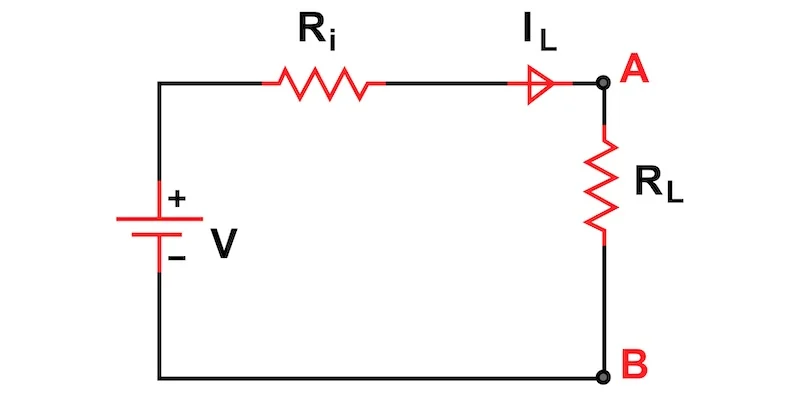
\includegraphics[width=0.5\textwidth]{figures/max_power_transfer_circuit.png}
            \caption{Maximum Power Transfer Theorem Circuit.}
            \label{fig:max_power_transfer_circuit}
        \end{figure}

        Giả sử chúng ta có một hệ thống với nguồn điện áp V có điện trở trong $R_i$ và cấp điện cho tải điện có điện trở $R_L$. 
        Định lý công suất cực đại sẽ được sử dụng để xác định giá trị điện trở tải $R_L$, 
        cho phép truyền công suất cực đại từ nguồn đến tải. 
        Công suất cực đại truyền đến tải phụ thuộc vào kích thước của điện trở tải.\par

        Từ mạch trong hình \ref{fig:max_power_transfer_circuit}, công suất truyền đến điện trở tải:
        \begin{equation}
            P = I_L^2 R_L = \frac{V^2 R_L}{(R_i + R_L)^2}
        \end{equation}

        Đối với công suất cực đại, chúng ta phân biệt phương trình trên với điện trở tải $R_L$ và coi kết quả bằng không. 
        Chúng ta sẽ có:
        \begin{equation}
            \frac{dP}{dR_L} = \frac{V^2 (R_i + R_L)^2 - 2R_L (R_i + R_L) V^2}{(R_i + R_L)^4} = 0 \Rightarrow R_L = R_i
        \end{equation}

        Lưu ý rằng công suất cực đại chỉ có thể được truyền từ nguồn đến tải khi điện trở trong của nguồn điện áp bằng điện trở của tải. 
        Việc khớp trở kháng đảm bảo rằng điện trở nguồn bằng điện trở tải. 
        Một điều nữa cần lưu ý là điện kháng tải cũng phải bằng giá trị âm của điện kháng nguồn để công suất cực đại được phản xạ ở phía tải điện. 
        Điều này có nghĩa là công suất tải chỉ có thể đạt cực đại khi trở kháng tải bằng liên hợp phức trở kháng nguồn.\cite{allaboutcircuits_impedance}

    \section{Công thức và mạch Impedance Matching}
        \begin{figure}[h]
            \centering
            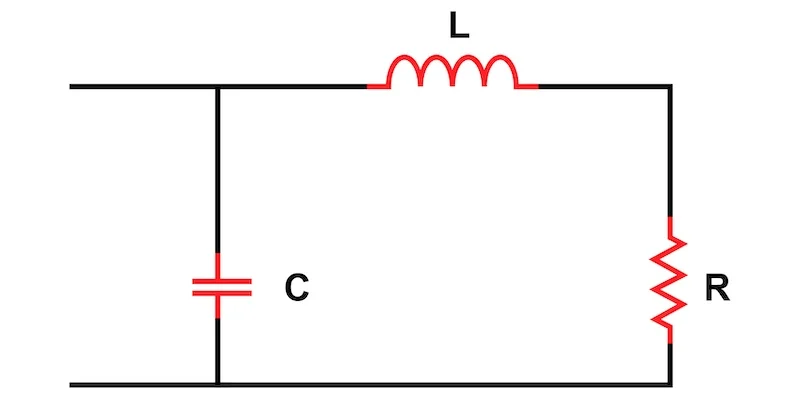
\includegraphics[width=0.5\textwidth]{figures/impedance_matching_circuit.png}
            \caption{Impedance Matching Circuit.}
            \label{fig:impedance_matching_circuit}
        \end{figure}

        Tính toán độ dẫn $Y_{in}$ cho mạch trên:
        \begin{equation}
            Z = \left(R + j\omega L\right) // \frac{1}{j\omega C}
        \end{equation}
        \begin{equation}
            Y_{in} = \frac{1}{Z} = j\omega C + \frac{1}{R + j\omega L}
        \end{equation}

        Sử dụng liên hợp phức và rút gọn phương trình trên:
        \begin{equation}
            Y = \frac{R}{R^2 + \left(\omega L\right)^2}
        \end{equation}
        \begin{equation}
            \omega_0 = \sqrt{\frac{1}{LC}} - \left(\frac{R}{L}\right)^2
        \end{equation}

        Ở tần số $\omega=0$, điện trở của $Y_{in}$ phải được đặt thành $R'$:
        \begin{equation}
            R' = R\left[1 + \left(\frac{\omega_0 L}{R}\right)^2\right]
        \end{equation}

        Đặt $\frac{\omega_0 L}{R}$ thành Q-factor:
        \begin{equation}
            R' = R\left[1 + Q^2\right]
        \end{equation}
        Từ các phương trình trên, ta có thể dễ dàng giải được bài toán phối hợp trở kháng trong bất kỳ mạch điện nào.\cite{allaboutcircuits_impedance}

    \section{Tầm quan trọng của Impedance Matching}
        Impedance matching cần được đảm bảo trong các thiết kế mạch tần số cao
        và mạch tốc độ cao. Nếu impedance trên đường tín hiệu bị sai lệch,
        khả năng cao xung sẽ bị méo và tín hiệu sẽ bị phản xạ.\par
        Mạch điện sẽ hoạt động tốt nhất khi có trở kháng phù hợp, nếu không, cả hệ thống sẽ hoạt động bất thường do hiệu ứng từ phản xạ tín hiệu.
        Sóng phản xạ sẽ gây ra độ trễ tín hiệu, làm méo pha, hay làm tín hiệu bị nhiễu.
        
    \section{Transformer impedance matching}

    \section{Transmission line impedance matching}
        Trên một transmission line, nếu đường truyền càng dài,
        sẽ có trở kháng đặc trưng của đường truyền khác nhau khác
        ở các khoảng cách khác nhau dọc theo transmission line.
        Nếu không thực hiện impedance matching, tín hiệu sẽ bị phản xạ
        và tạo ra sóng dừng.

    \section{Antenna impedance matching}

    \section{Impedance matching trong mạch RF}
        không biết cái hình để làm gì nên để tạm\cite{cadence_impedance}
        \begin{figure}[h]
            \centering
            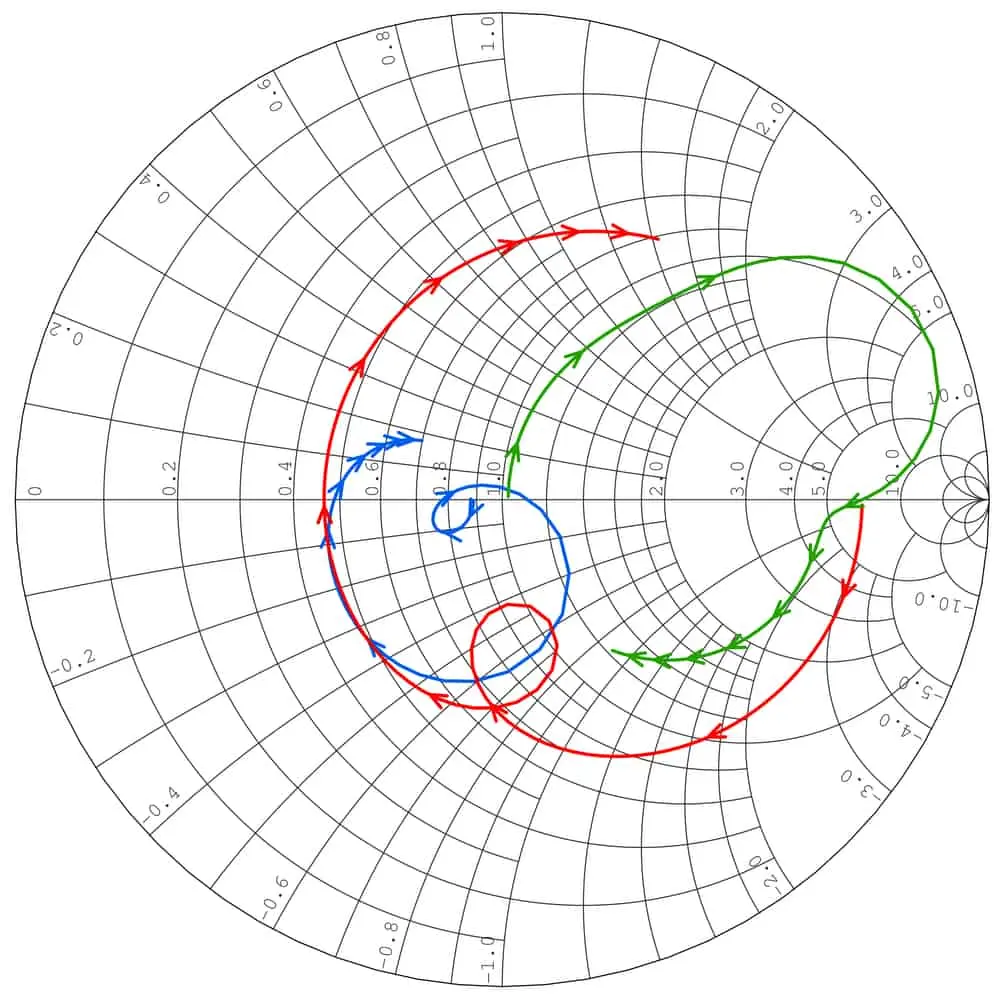
\includegraphics[width=0.5\textwidth]{figures/smith_chart.png}
            \caption{Smith charts are one of the traditional methods used for developing impedance-matching networks for RF circuits}
            \label{fig:smith_chart}
        \end{figure}

    \section{Conjugate Matching}
    \section{Reflectionless Matching}
    \cite{cadence2021conjugatematching}